\section{Model used to explore the parameters}
In this part, I use HIFI as an example.
My goal is to show where each standing wave in HIFI is born.

\begin{figure}
    \centering
    %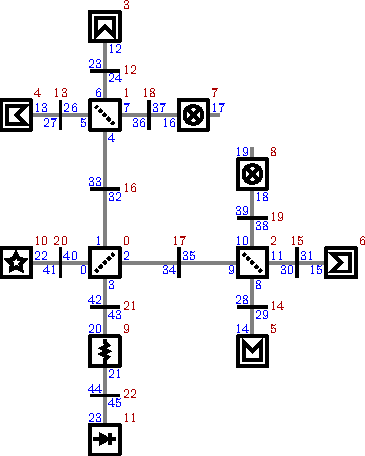
\includegraphics{ports_diplexerband}
\end{figure}

\section{Folding and calibration}

We are going to assume that the intrinsic sideband ratio of the mixer is 0.5, that is that the mixer is perfectly balanced.  This is of course not the case, but our goal here is to explore the effect of the standing waves on the coupling, not the imperfections of the mixer.

\section{Exploration}

At first, the whole system will be as perfect as I can make it.  I do not have a model for a perfect grid, but I can make the grid so thin and dense that it will drown the effect of the grid within the thickness of the line in the plots.

Then, little by little I will make the elements more realistic, and describe the results.

Each time, I present a plot of
\begin{itemize}
    \item the coupling of the mixers to the LO before mixing,
    \item the coupling of the mixers to the sky before mixing,
    \item the coupling of the mixers to the LO after mixing,
    \item the coupling of the mixers to the sky after mixing,
    \item the sideband ratio of the LO.
    \item the sideband ration of the sky.
\end{itemize}
\todo[inline]{
    Whenever possible, I must refer to HIFI data exhibiting this kind of feature.
}

Why do the LO coupling matters?
Because the LO is a source of noise.
And a strong one, think \SI{120}{\kelvin}.
Of course, diplexer bands and beam splitter bands try to minimize the LO coupling, but even \SI{1}{\percent} of \si{120}{\kelvin} matters, remember that the CMB is at \SI{3}{\kelvin}.
Note that this value must be divided by 2: it radiates \SI{120}{\kelvin}, but only half of it goes through the H or V grid, therefore it shines at \SI{60}{\kelvin} in each.


Wait.  How do I model a incoherent source with a coherent one?
Is a \SI{10}{\kelvin} source radiating \SI{10}{\kelvin} in H and \SI{10}{\kelvin} in V?
The temperature scale is a little bit weird.  Or is it 5 in each?

At a given time, are the H and V components of a wave correlated?  Well, yes, they are.
I must send diagonal polarizations through the grids instead of assuming that H and V are not locked.  They are phase-locked, they have the same frequency.  For the sky that's kinda easy, I just send a 45 degrees signal.  What about the relative phase between the two?  How do I model that?  Thing is, H anv V is totally arbitrary.

Any wave can be seen as a combination of two polarizations.  That's true.  My problem
is that the relative phase between these two polarizations is a-priori random.  And it changes with time.  But the changes are slow.
How slow are they?  Well, we're integrating for 1 to 4 seconds.  That is a LOT of time.
The coherence time of the instrument is much shorter than that.  This means that the relative phase changes randomly a lot between H and V for the time of an integration.  Or, in other terms, I don't have to care.

Now, this poses the problem of cross-talk, doesn't it?  Well, not really.  Because cross-talk is phase-locked.  Some H goes to V, but it's still originating from H so it counts.  What doesn't count, when averaging over a long observation, is the real V onto the real H.

\subsection{Entry grid}
We have to expect a slightly different H/V ratio on each side of the grid.
Plus, the amount of power may be different too.

By zooming on the Y axis of the plots, I show that the higher the frequency, the more the grid leaks.  This is not surprising.

\subsection{Perfect instrument}
Even in the perfect case, the diplexer is optimally tuned to the center of the IF, and there is a twenty-percent degradation of the coupling at the borders of the IF.

Show that there is a slight offset of the perfect diplexer tuning due to the entry grid not being perfect.

This means that we are correct in taking calibration measures in order to tune the diplexer instead of relying on the value given by the formula.

\begin{figure}
    \centering
    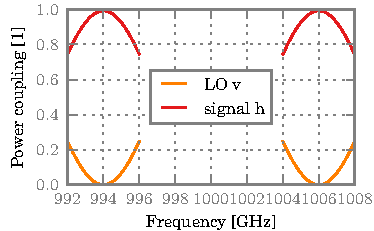
\includegraphics{chapter_3/0_ideal_h_dsb}
    %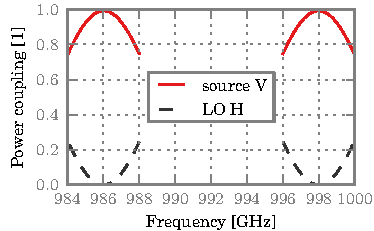
\includegraphics{chapter_3/0_ideal_v_dsb}
\end{figure}

\subsection{Reflective co-pol mixer}
Turning on the co-pol reflectivity of the mixer simulates the imperfection of the horn.

\subsection{Reflective cross-pol mixer}
This simulates a desired behavior of the horn: the crosspol must not couple to the mixer.
Well, it would be nice if the crosspol would just disappear, but it is not how rectangular horns work, they reflect what they don't want.

\subsection{Reflective co- and cross-pol, standing waves}
As soon as one reflection is turned on, we observe a standing wave pattern.
This is a priori paradoxical.
Indeed, for standing waves to appear, a cavity must exist, that means we need two reflective surfaces and we have only one.

We show that the mixer is actually looking at itself through the leaky grid of the diplexer unit.

\subsection{Blaming the grids}
We make the grid much thinner and denser, and the standing wave patters from the previous subsection disappears.

We make the grid coarser and it gets worse.

There is a limit on how coarse you can make the grid, as the grid model my Houde makes assumptions on the radius of the wires, their spacing, and the wavelength.

With insanely bad grids, we show that the standing wave pattern is actually far from sinusoidal, as the cavity has a very high Q.

\subsection{Imperfect rooftop mirrors}
This is how we can achieve the first exchange of polarization power.
Indeed, if we make only the co-pol of the mixer reflective, with an imperfect roof-top mirror we observe standing wave patters on the two polarizations.

We can also observe a beat of the standing wave patterns.  This is due to the two arms of the diplexer units being of different length.  A fourrier transform can reveal two picks.
In fact, every cavity involving the diplexer will show these picks.

\subsection{Turn on the LO reflection}
This creates a very strong modulation on top of all the others.
This also allows the two mixers to see each other.
Indeed, because the entry grid leaks, some standing wave patters in one polarization will affect the other after reflection on the local oscillator.

\subsection{Effect of the attenuator in front of the local oscillator}
Reduces the cross talk and the LO standing waves.

\subsection{Simulated diplexer scans}
These reproduce distorsions observed on real diplexer scans.

\subsection{Influence of the diplexer tuning on the cross talk}
Show that mistuning one diplexer has an effect on the coupling of the mixer in the other branch.
